%!TEX root = ../main.tex
\section{Giới thiệu}

\begin{frame}{Ý tưởng chính của tiến hóa đa nhiệm}
    \begin{columns}
        \begin{column}{0.45\textwidth}
            \begin{block}{Ý tưởng}
                \begin{figure}
                    \centering
                    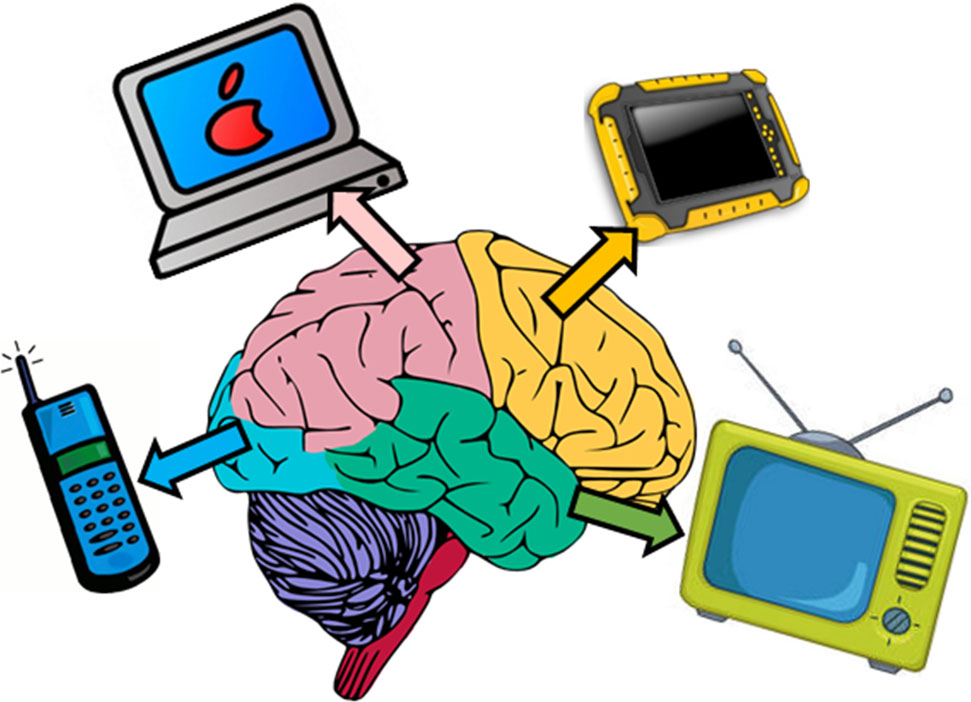
\includegraphics[width=0.7\linewidth]{figure/introduction/cognitive_multitasking.png}
                    \caption{Khả năng đa nhiệm của con người}
                    \label{fig:introduction:human_multitask}
                \end{figure}
            \end{block}
            \begin{block}{Xu hướng}
                Thuật toán mô phỏng trí thông minh trong tự nhiên.
            \end{block}
        \end{column}
        \begin{column}{0.5\textwidth}  %%<--- here
            \begin{block}{Thuật toán tiến hóa đa nhiệm}
                \begin{figure}
                    \centering
                    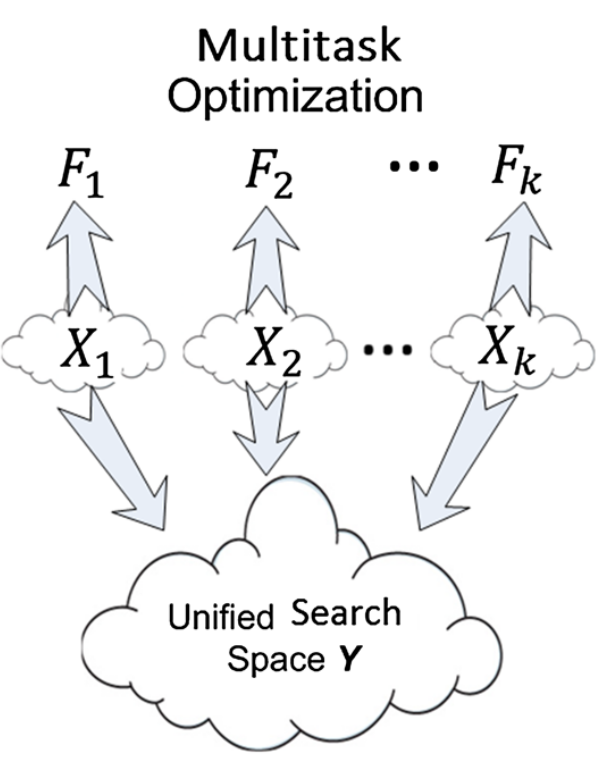
\includegraphics[width=0.5\linewidth]{figure/introduction/mto.png}
                    \caption{Tiến hóa đa nhiệm mô phỏng lại khả năng giải quyết nhiều việc cùng một thời điểm của con người}
                    \label{fig:introduction:mto}
                \end{figure}
            \end{block}
        \end{column}
    \end{columns}
\end{frame}

\begin{frame}{Ứng dụng nổi bật của tiến hóa đa nhiệm}
    \begin{block}{Tối ưu tại cloud computing}
        \begin{figure}
            \centering
            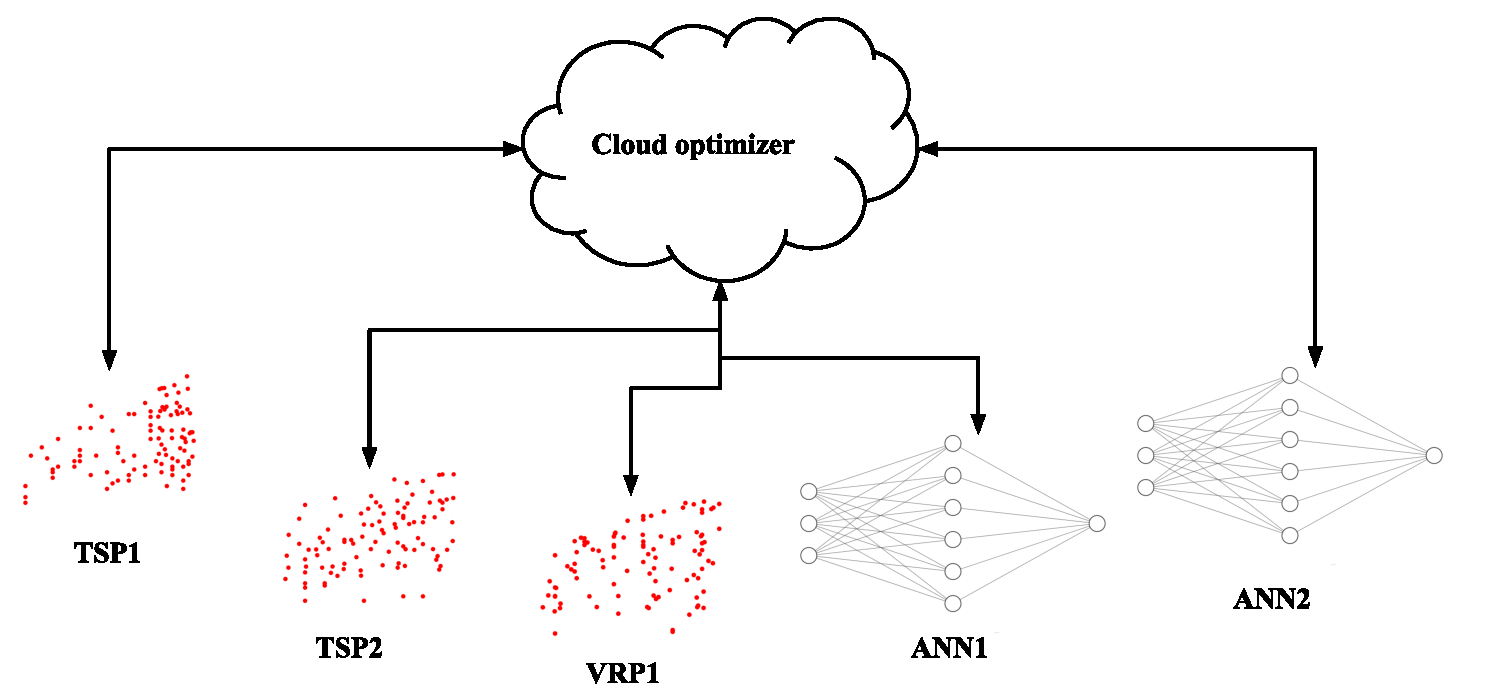
\includegraphics[width=0.7\linewidth]{figure/introduction/cloud_optimizer.eps}
            % \caption{Cloud optimizer}
            % \label{fig:introduction:cloud_optimizer}
        \end{figure}
    \end{block}
    \begin{block}{Các nghiên cứu đã áp dụng tiến hóa đa nhiệm}
        \begin{itemize}
            \scriptsize
            \item \fullcite{binh2018effective}
            \item \fullcite{chandra2018evolutionary}
        \end{itemize}
    \end{block}
    % Một hình minh họa giải nhiều TSP ở nhiều map khác nhau chia sẻ lẫn nhau.
    % Nhớ nói là chỉ đưa ra ví dụ, không đào sâu nghĩ bài toán.
    % Bài TSP thì có 
    % Cite vài bài của nhóm anh Thành.
    % Một hình minh họa bài giải nhiều ANN cho bộ UCI của chandra.
    % Suy ra ứng dụng Optimization on Cloud của ông Ong.
\end{frame}

\begin{frame}{Câu hỏi nghiên cứu còn tồn tại}
    \begin{columns}
        \begin{column}{0.45\textwidth}
            \begin{block}{Các tồn tại của các nghiên cứu trước}
                \begin{itemize}
                    \item Ứng dụng hướng đến làm thuật toán tối ưu trên cloud.
                    \item Cloud có \textbf{số lượng người dùng lớn}.
                    \item Chỉ thử nghiệm và chứng minh tính hiệu quả trên tập hợp \textbf{2 đến 3 tác vụ}.
                \end{itemize}
            \end{block}
            \begin{block}{Yêu cầu}
                \begin{itemize}
                    \item Thiết kế thuật toán chạy tốt với số lượng lớn tác tác vụ.
                    \item Thuật toán có ít tham số.
                \end{itemize}
            \end{block}
        \end{column}
        \begin{column}{0.45\textwidth}
            % \begin{exampleblock}{Hướng giải quyết chung}
            %     \begin{itemize}
            %         \item Thay vì cho tất các tác vụ kết hợp với nhau, chỉ ghép các tác vụ hỗ trợ được cho nhau được kết hợp với nhau.
            %         \item Ghép cặp dựa trên phân tích dữ liệu sinh ra trong quá trình tối ưu.
            %     \end{itemize}
            % \end{exampleblock}
            \begin{exampleblock}{Hướng giải quyết cụ thể}
                \begin{itemize}
                    \item Thiết kế \textbf{cấu trúc mới} cho tiến hóa đa nhiệm phù hợp với tối ưu nhiều tác vụ.
                    \item Áp dụng mô hình \textbf{Multi-Armed Bandits}, học trên dữ liệu hàm mục tiêu để ghép cặp các tác vụ
                \end{itemize}
            \end{exampleblock}
        \end{column}
    \end{columns}
    % Cloud nên phải có nhiều tác vụ hơn 2 hoặc ba vì nhiều người dùng, tìm hình minh họa.
    % Yêu cầu của thuật toán mới: nhiều tác vụ, ít tham số, phụ thuộc dữ liệu tối ưu.
    % Suy ra -> đề xuất thuật toán mới là gì.
\end{frame}